% !TeX spellcheck = pt_BR

%%%%%%%%%%%%%%%%%%%%%%%%%%%%%%%%%%%%%%%%%%%%%%%
% Modelo adaptado do template original de
% Ted Pavlic (http://www.tedpavlic.com)
% Todos os créditos a ele.
%
% Na versão atual, o que foi modificado
% do original:
% Ajusta a numeração das questões e
% passa para português.
% Além de separar as configurações
% em um arquivo .cls separado.
%
% Crédito ao Roberto por ter feito
% a maior parte do trabalho de passar
% para o português e fazer outros
% ajustes para a versão atual deste template.
%%%%%%%%%%%%%%%%%%%%%%%%%%%%%%%%%%%%%%%%%%%%%%%


%----------------------------------------------------------------------------------------
%	PACKAGES E OUTRAS CONFIGURAÇÕES
%----------------------------------------------------------------------------------------

\documentclass{homeworkclass}

\usepackage{animate}


\usepackage{myMacros}


\hmwkTitle{Lista\ de\ Exercícios \#1}
\hmwkDueDate{Quinta,\ 04\ de\ Julho,\ 2019}
\hmwkClass{Elementos de Processamento de 	Sinais}
\hmwkClassTime{Segundas e Quartas: 08:00--10:00}
\hmwkClassInstructor{Prof.\ Sergio Lima Netto}
\hmwkAuthorName{Vinicius Mesquita de Pinho}
\hmwkAuthorShortName{Vinicius Mesquita}

\begin{document}

\maketitle

%----------------------------------------------------------------------------------------
%	SUMÁRIO
%----------------------------------------------------------------------------------------

%\setcounter{tocdepth}{1} % Uncomment this line if you don't want subsections listed in the ToC

\clearpage
\newpage
%\tableofcontents
%\newpage

%----------------------------------------------------------------------------------------
%	QUESTÃO 1
%----------------------------------------------------------------------------------------

% To have just one problem per page, simply put a \clearpage after each problem

\begin{homeworkProblem}

	Primeiro, geramos uma senoide com frequência de $f_{c} = 80$~Hz, amostrada com frequência $f_{s} = 1$~kHz. A mesma pode ser vista na Figura~\ref{fig:sine}. 
	
	O nosso sinal é então: 
	\begin{equation*}
	x(n) = \sin(\theta) = \sin(2 \pi f_{c}n).
	\end{equation*}

\begin{figure}[!ht]
	\centering
	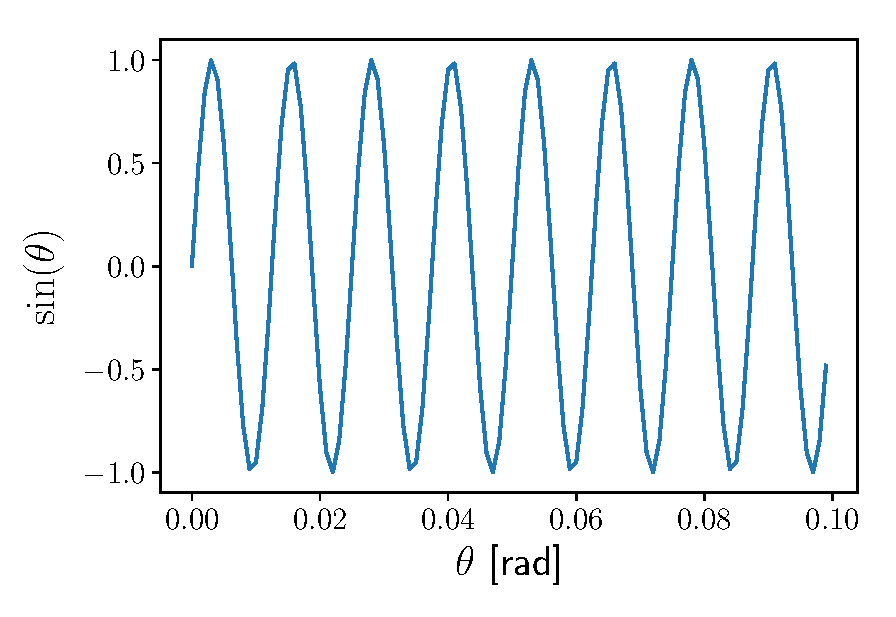
\includegraphics[width=0.6\linewidth]{figs/sine}
	\caption{Seno em função do ângulo $\theta$, representado de 0 a $0.1$ radianos.}
	\label{fig:sine}
\end{figure}

	
	O próximo passo foi gerar um ruído gaussiano. Como uma espécie de teste de sanidade, temos o histograma apresentado na Figura~\ref{fig:gaussiannoise}. A curva vermelha foi plotada a partir da equação da PDF da Gaussiana, e podemos verificar visualmente que os dados gerados em azul seguem a uma distribuição normal.	
	
	O ruído será representado por $\zeta(n)$.
	
	\begin{figure}[!ht]
		\centering
		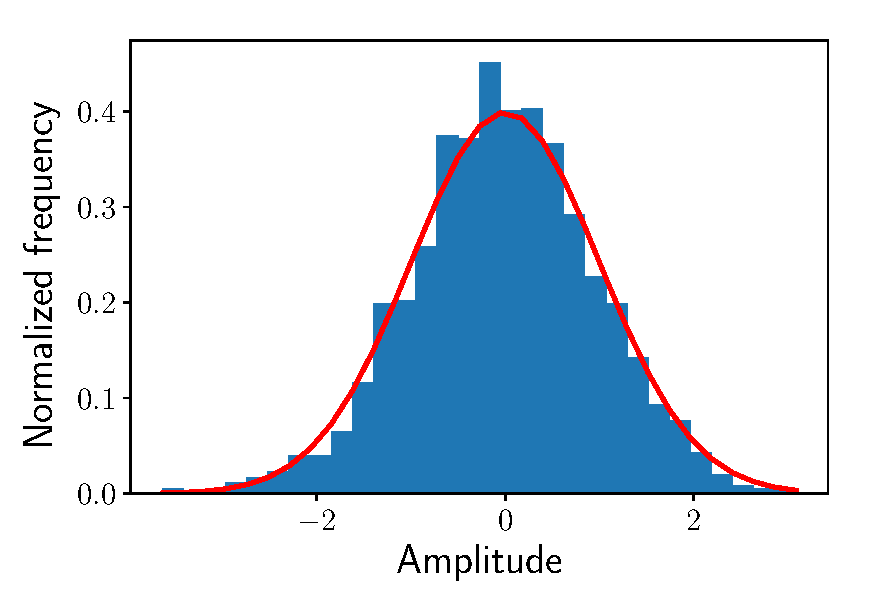
\includegraphics[width=0.6\linewidth]{figs/gaussian_noise}
		\caption{Histograma do ruído gaussiano gerado.}
		\label{fig:gaussiannoise}
	\end{figure}

	A Figura~\ref{fig:sineandnoise} é o resultado de $x(n)$ da Figura~\ref{fig:sine} e do ruído representado no histograma da Figura~\ref{fig:gaussiannoise}. A operação pode ser escrita como:
	\begin{equation*}
	y(n) = x(n) + \zeta(n).
	\end{equation*}
	
	Colocamos uma ganho $k = 0.2$ para demonstrar o resultado da adição do ruído e ainda conseguirmos visualizar a senoide, dada a amplitude do ruído $\zeta(k)$ como vista na Figura~\ref{fig:gaussiannoise}.
	\begin{figure}[!h]
		\centering
		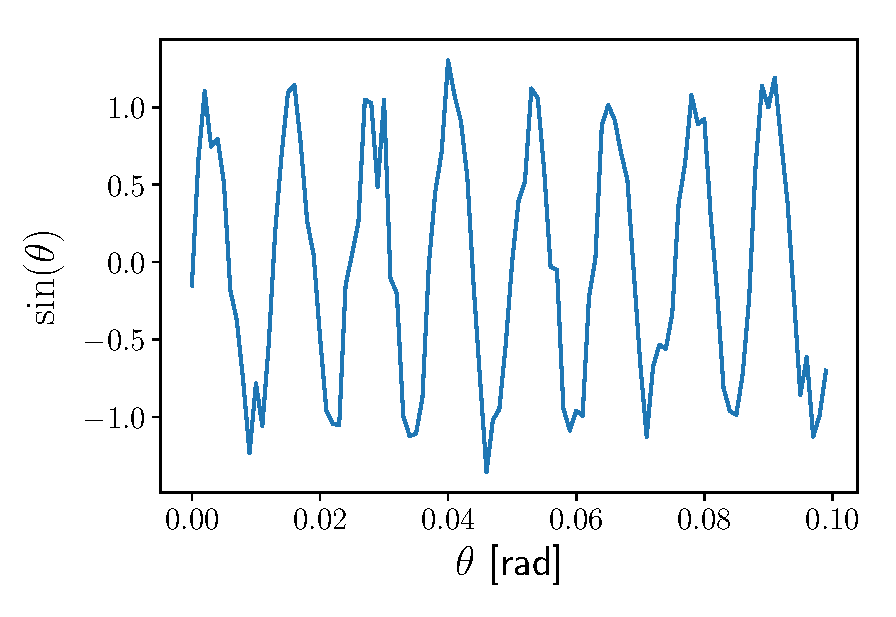
\includegraphics[width=0.6\linewidth]{figs/sine_and_noise}
		\caption{Função seno adicionada do ruído gaussiano. O ganho no ruído neste caso é de $k = 0.2$.}
		\label{fig:sineandnoise}
	\end{figure}

	Sendo a DFT de $y(n)$ expressa como: 
	\begin{equation}\label{eq:dft}
	Y(m) = \sum_{l=0}^{L - 1} y(l) W^{li}_L, ~\textrm{para}~ 0 \leq m \leq L - 1,
	\end{equation}
	na Figura~\ref{fig:dft} temos a parte positiva $|Y(f)|$, onde $f$ é a frequência em Hz, que relaciona-se com $m$ da equação \eqref{eq:dft} por $f = f_{s}\frac{L-1}{L}m$. 

	Para obtermos uma estimativa da frequência $f_{c}$ da senoide $x(n)$, analisar de forma visual e verificar que em $f = 80$~Hz encontra-se um pico de $|Y(f)|$.
	\begin{figure}[!ht]
		\centering
		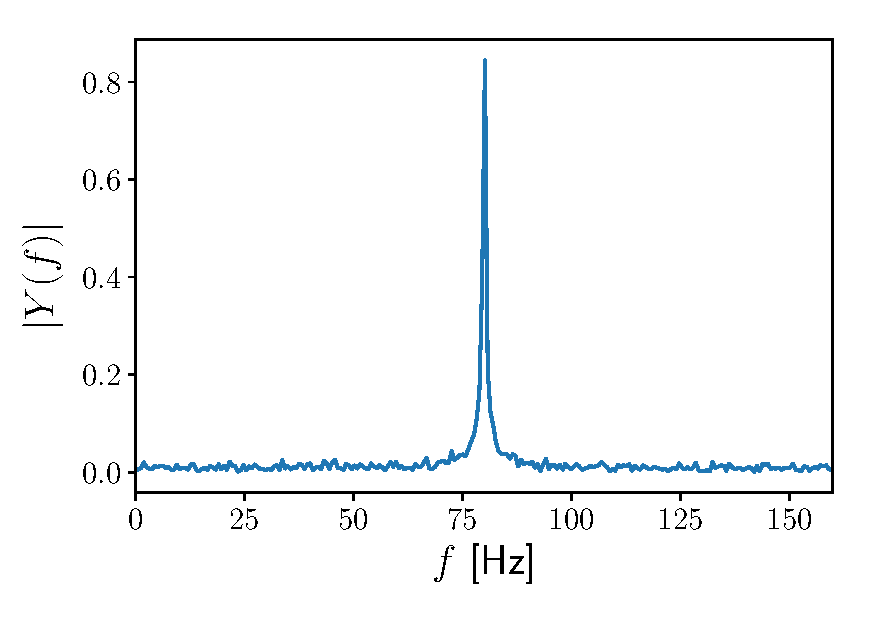
\includegraphics[width=0.7\linewidth]{figs/dft}
		\caption{Módulo da DFT do sinal adicionado de ruído.}
		\label{fig:dft}
	\end{figure}
	Para automatizarmos o processo, podemos construir um algoritmo que identifique o máximo de $|Y(f)|$ e nos retorne em qual $f$ ele ocorre. Para o exemplo ilustrado, a resposta foi $\hat{f_c} = 80.2$~Hz.
	
	Porém este algoritmo nem sempre nos informará uma resposta correta. Quando o ganho $k$ do ruído aumenta perdemos a referência do pico, como podemos ver na Figura~\ref{fig:ruidera}. Portanto, a estimação da frequência por este meio não traz um resultado satisfatório quando o ruído tem uma amplitude tão grande quanto o pico do valor absoluto da DFT.
	
	\begin{figure}[!h]
		\centering
		\subfloat[$k = 1$, $\hat{f_c} = 80.08$~Hz]{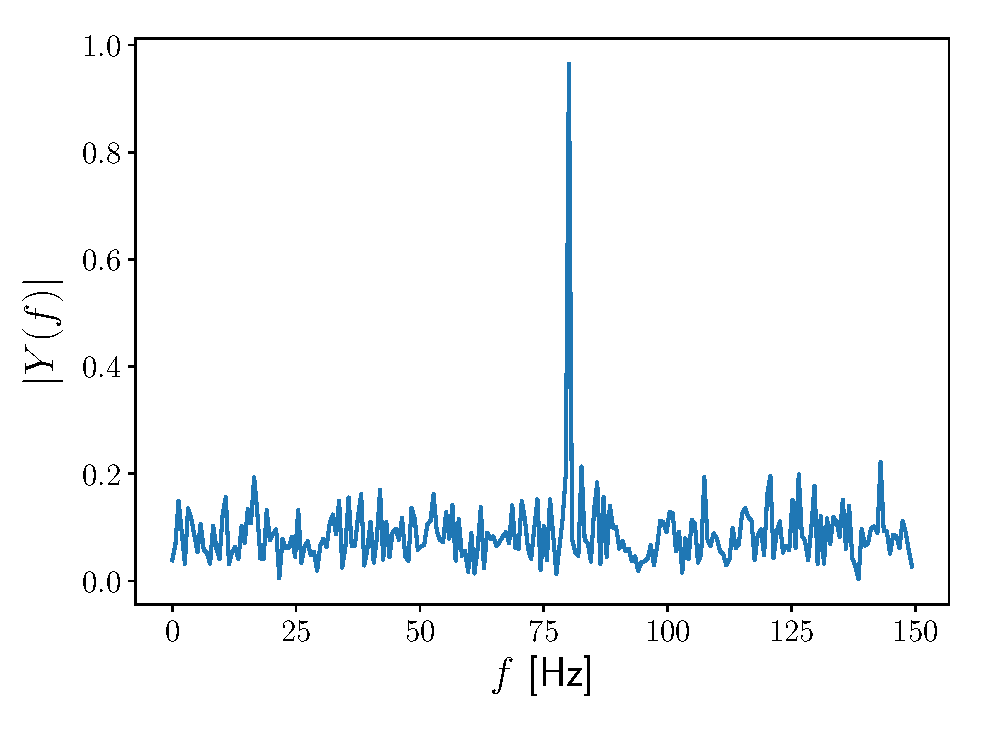
\includegraphics[width=0.5\linewidth]{figs/dft-1}\label{fig:k_1}}
		~
		\subfloat[$k = 2$, $\hat{f_c} = 80.08$~Hz]{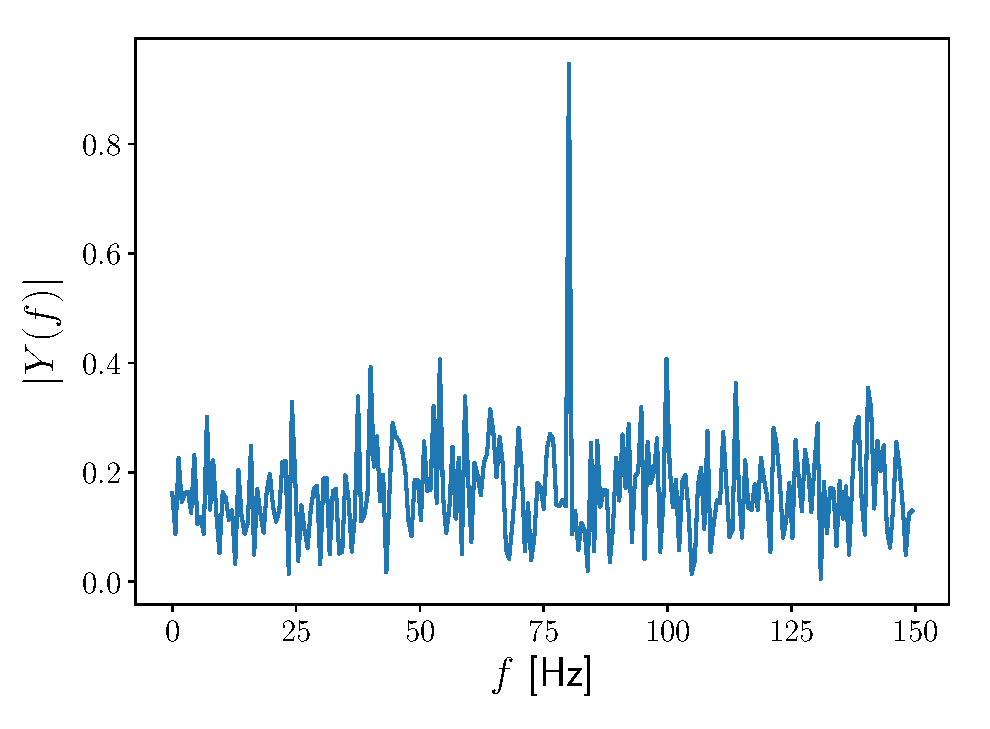
\includegraphics[width=0.5\linewidth]{figs/dft-2}	\label{fig:k_2}}
		\\
		\subfloat[$k = 5$, $\hat{f_c} = 88.98$~Hz]{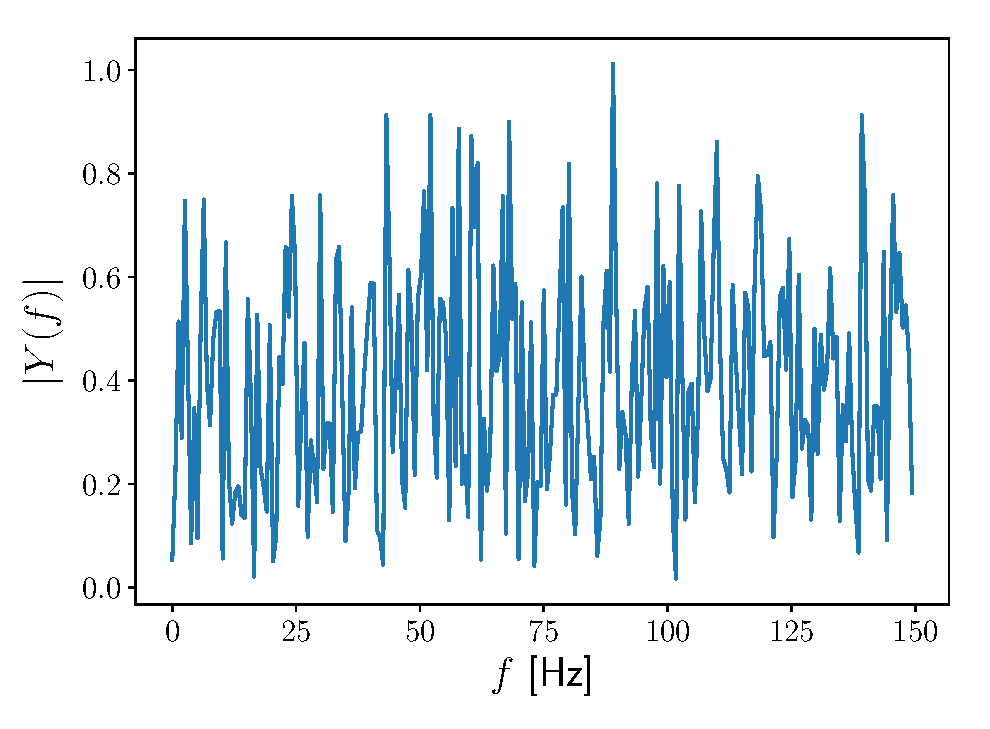
\includegraphics[width=0.5\linewidth]{figs/dft-5}	\label{fig:k_5}}
		~
		\subfloat[$k = 10$, $\hat{f_c} = 107.42$~Hz]{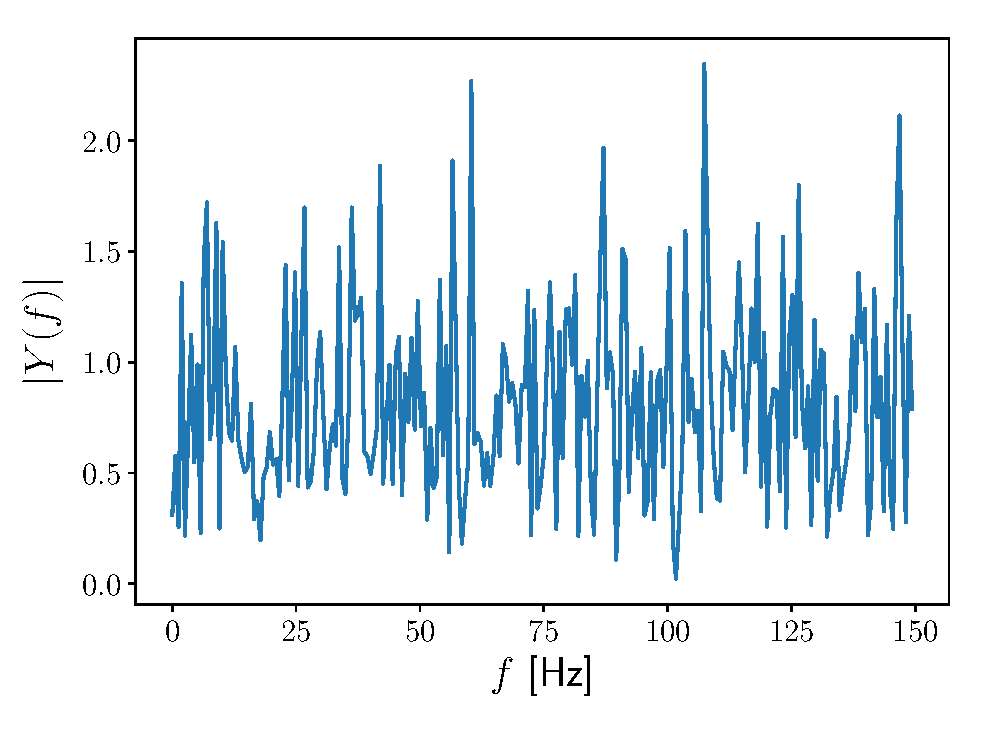
\includegraphics[width=0.5\linewidth]{figs/dft-10}	\label{fig:k_10}}
		
		\caption{Efeito do aumento do ganho do ruído $k$ na estimativa $\hat{f_c}$ da frequência da senoide.}
		\label{fig:ruidera}
	\end{figure}

	Para resolvermos este problema, podemos fazer um pré-processamento no sinal recebido, como por exemplo fazer um realce do sinal desejado com um filtro levando em conta a estatística do ruído e a correlação do mesmo com o sinal. Depois do realce do sinal, podemos assim estimar sua a frequência da portadora.
	
\end{homeworkProblem}

\cleardoublepage
\begin{homeworkProblem}
	
	Para este exercícios, vamos definir dois vetores:
	\begin{equation*}
	\xbf = [1 \quad 2]^{\Trm} \qquad
	\hbf = [1 \quad 0]^{\Trm}
	\end{equation*}
	O tamanho os dois é de $L_{x} = L_{h} = 2$. Portanto, é de se esperar que a convolução entre os dois sinais tenha um tamanho $L_{y} = L_{x} + L_{h} - 1 = 3$.
	
	Usando a função do Numpy chamada convolve, o resultado que nos é apresentado é:
	\begin{equation*}
	\ybf = \xbf * \hbf = [1 \quad 2 \quad 0]^{\Trm}. 
	\end{equation*}
	Portanto, $L_{y}$ de fato é 3.
	
	Podemos também fazer a conta escrevendo $\xbf$ como uma matriz Toeplitz, que fica com a forma:
	\begin{equation*} \Xbf = 
	\begin{bmatrix}
	1 & 0 \\ 
	2 & 1 \\ 
	0 & 2
	\end{bmatrix} 
	\end{equation*}
	Ao fazermos $\ybf = \Xbf\hbf$ temos:
	\begin{equation*}
	\ybf = \Xbf\hbf = 	\begin{bmatrix}
	1 & 0 \\ 
	2 & 1 \\ 
	0 & 2
	\end{bmatrix} 	\begin{bmatrix}
	1  \\ 
	0	\end{bmatrix} = \xbf * \hbf = \begin{bmatrix}
	1 \\ 
	2 \\ 
	0 
	\end{bmatrix} 
	\end{equation*}
	
	Também podemos fazer essas mesmas operações no domínio da frequência. Primeiro, vamos explorar o caso em que não fazemos o \textit{zero-padding}.
	Também analisaremos o caso em que temos $\xbf$ e $\hbf$ tais que:
	\begin{equation*}
	\xbf = [1 \quad 2]^{\Trm} \qquad
	\hbf = [1 \quad 0]^{\Trm}
	\end{equation*}
	Usando a função \textit{fftconvolve} do Scipy como um \textit{sanity check}, o resultado é:
	\begin{equation*}
	\ybf^\prime = \begin{bmatrix}
	1 \quad 2
	\end{bmatrix}^{\Trm}.
	\end{equation*}
	Agora vamos fazer de outra forma. Vamos calcular a DFT de $\xbf$ e de $\hbf$, multiplicá-los e calcular a IDFT do resultado.
	
	Para ambos, a matriz de DFT é: 
	\begin{equation*} \Wbf_{2} = 
	\begin{bmatrix} 
	1 & 1 \\ 
	1 & -1
	\end{bmatrix}.
	\end{equation*}
	Então temos:
	\begin{equation*}
	\Xbf^{\prime} = \Wbf_{2}\xbf = 	\begin{bmatrix} 
	                        3 \\ 
	                        -1
	                        \end{bmatrix}
	\end{equation*}
	e
		\begin{equation*}
	\Hbf^{\prime} = \Wbf_{2}\hbf = 	\begin{bmatrix} 
									1 \\ 
									1
									\end{bmatrix}.
	\end{equation*}
	Portanto,
	\begin{equation*}
	\Ybf^{\prime} = \Xbf^{\prime}\odot\Hbf^{\prime} = \begin{bmatrix} 
	3 \\ 
	-1
	\end{bmatrix}.
	\end{equation*}
	Agora, para fazermos a IDFT, a matriz será:
	\begin{equation*} \Wbf_{2}^{-1} = 
		\begin{bmatrix} 
	0.5 & 0.5 \\ 
	0.5 & -0.5
	\end{bmatrix}.
	\end{equation*}
	Portanto:
	\begin{equation*}
	\ybf^{\prime} = \Wbf_{2}^{-1} \Ybf^{\prime} = \begin{bmatrix} 
													1 \\ 
													2
													\end{bmatrix}.
	\end{equation*}
	Ok, este resultado não é esperado para a convolução linear. Para atingirmos o resultado esperado para convolução linear é necessário fazermos o \textit{zero-padding}. Neste caso, como resultado da convolução linear tem que ter tamanho $L_{y} = 3$, os dois vetores vão ser acrescidos de $1$ zero no final. Portanto, teremos:
	\begin{equation*}
	\xbftil = [1 \quad 2 \quad 0]^{\Trm} \qquad
	\hbftil = [1 \quad 0 \quad 0]^{\Trm}
	\end{equation*}
	Usando agora a função \textit{fftconvolve} do Scipy, temos o resultado esperado:
	\begin{equation*}
	\ybf = [1 \quad 2 \quad 0]^{\Trm}. 
	\end{equation*}
	Fazendo novamente o cálculo pela matriz de DFT. A matriz $\Wbf_{3}$ neste caso é:
	\begin{equation*} \Wbf_{3} = 
	\begin{bmatrix} 
	1  & 1 & 1 \\ 
	1 & -0.5-\jrm0.866 & -0.5+\jrm0.866 \\
	1 & -0.5+\jrm0.866 & -0.5-\jrm0.866	
	\end{bmatrix}
	\end{equation*}
	
	Então temos:
	\begin{equation*}
	\tilde{\Xbf} = \Wbf_{3}\xbftil = 	\begin{bmatrix} 
	3 \\ 
	-\jrm1.732 \\
	+\jrm1.732
	\end{bmatrix}
	\end{equation*}

	\begin{equation*}
	\tilde{\Hbf} = \Wbf_{3}\hbftil = 	\begin{bmatrix} 
	1 \\ 
	1 \\ 
	1 
	\end{bmatrix}.
	\end{equation*}
	Portanto,
	\begin{equation*}
	\tilde{\Ybf} = \tilde{\Xbf} \odot \tilde{\Hbf} = \begin{bmatrix} 
	3 \\ 
	-\jrm1.732 \\
	+\jrm1.732
	\end{bmatrix}.
	\end{equation*}
	Agora, para fazermos a IDFT, a matriz será:
	\begin{equation*}  \Wbf_{3}^{-1} = 
	\begin{bmatrix} 
	1/3  & 1/3 & 1/3 \\ 
	1/3 & -1/6 +\jrm0.289 & -1/6-\jrm0.289 \\
	1/3 & -1/6 -\jrm0.289 & -1/6+\jrm0.289	
	\end{bmatrix}
	\end{equation*}
	Portanto:
	\begin{equation*}
	\ybf = \ybftil = \Wbf_{3}^{-1} \tilde{\Ybf} = \begin{bmatrix} 
	1 \\ 
	2 \\
	0
	\end{bmatrix}.
	\end{equation*}	
	
	
	
\end{homeworkProblem}

%----------------------------------------------------------------------------------------
%	QUESTÃO 1
%----------------------------------------------------------------------------------------

\end{document}